\documentclass{article}
\usepackage{graphicx}
\usepackage{hyperref}
\usepackage{fancyhdr}
\usepackage{indentfirst}
\usepackage{graphicx}
\usepackage{newlfont}
\usepackage{amssymb}
\usepackage{amsmath}
\usepackage{latexsym}
\usepackage{lipsum}
\usepackage{tikz}
\usepackage{amsthm}
\usepackage{algorithm}
\usepackage{algpseudocode}
\usepackage{stmaryrd}
\usepackage{listings}
\usepackage{xcolor}
\usepackage{xcolor, colortbl}
\usepackage{pgfgantt}
\usepackage{graphicx}
\usepackage{dirtree}
\usepackage{todonotes}

\usetikzlibrary{automata,arrows}
\pgfmathtruncatemacro\distance{1}

\definecolor{green}{rgb}{0,0.5,0}
\definecolor{red}{rgb}{1,0,0}
\definecolor{yellow}{rgb}{0.5,0.5,0}
\definecolor{codeashgrey}{rgb}{0,0.6,0}
\definecolor{codegray}{rgb}{0.5,0.5,0.5}
\definecolor{codepurple}{rgb}{0.58,0,0.82}
\definecolor{backcolour}{rgb}{0.95,0.95,0.92}
\definecolor{ashgrey}{rgb}{0.7, 0.75, 0.71}

\lstdefinestyle{mystyle}{
    backgroundcolor=\color{backcolour},   
    commentstyle=\color{codeashgrey},
    keywordstyle=\color{magenta},
    numberstyle=\tiny\color{codegray},
    stringstyle=\color{codepurple},
    basicstyle=\ttfamily\footnotesize,
    breakatwhitespace=false,         
    breaklines=true,                 
    captionpos=b,                    
    keepspaces=true,                 
    numbers=left,                    
    numbersep=5pt,                  
    showspaces=false,                
    showstringspaces=false,
    showtabs=false,                  
    tabsize=2
}

\lstset{style=mystyle}

\theoremstyle{definition}
\newtheorem{definition}{Definition}[section]

\theoremstyle{definition}
\newtheorem{exmp}{Example}[section]

\title{Final report: Extract Choreography Automata for Program Understanding}
\author{Student: Gabriele Genovese\\Supervisor: Cinzia Di Giusto}
\date{\today}

\begin{document}

\maketitle


\section*{Abstract}
The recent development of concurrent and distributed applications has raised new
interest in programming paradigms incorporating threads and message passing into
their logic. The use of choreographies
%which are behavioral types, 
can ensure some typical properties of concurrent systems (such as liveness, lock
freedom and deadlock freedom). ChorEr is a preliminary static analysis tool for
a fragment of Erlang programs that generates choreography automata. We plan to
build on the existing tool to implement new functionalities and cover more
primitives, thus extending the expressiveness of the language under consideration.

\newpage

\tableofcontents

\newpage

\section{Introduction}
The rise of service computing and microservices led to a shift from  
monolithic apps to distributed components using message-passing.  
%  
In this field, \emph{choreographic} coordination~\cite{WS-CDL} lets  
designers focus on \emph{application-level protocols}, i.e., a  
description of \emph{communication interactions}\footnote{%  
  An interaction is a full message-passing event, including both  
  sending and receiving.} among system components (called  
\emph{participants}).
%
This focus is typically expressed by two distinct, yet related views
of distributed computations: the so-called \emph{global} and
\emph{local} views.
%
The former view abstracts away from the actual communication
infrastructure in order to give a blueprint of the communication
protocol.
%
The latter view provides the description of the communication
behavior of participants in isolation and can guide their
implementation.
Choreographies can be expressed in modeling languages or formalism
(like WS-CDL~\cite{WS-CDL}, BPMN diagrams~\cite{BPMN}),
multiparty session types~\cite{HondaYC16}, message-sequence charts,
multiparty contracts, and many others (see also the survey
in~\cite{Huttel+16}).

Besides offering a suitable development for message-passing systems,
global views yield a high-level description of application-level
protocols.\footnote{According to the so-called top-down approach, a
  global view (formalized, e.g., as a multiparty session type) can be
  algorithmically projected on a local view preserving relevant
  properties.}
%
It is therefore crucial that global views faithfully capture
all the interactions in the system.
%
While this is relatively simple to guarantee when participants'
implementations are driven by the global view (e.g., in the top-down
approach), the correspondence can be easily spoiled when software
evolves or dynamic  composition  takes place (as advocated in
microservices architectures).
%
The classical top-down approach is then of little help: one needs to
write a global description of the desired behavior and then use type
checking or monitoring to find possible discrepancies.

Instead, we aimed to explore the concept of a \textit{bottom-up approach}.  
Bottom-up methods (such as \cite{myh09,lt12,lty15,cflm17,cms18}) focus on  
"extracting" global views from existing code. This is particularly useful  
when no pre-existing global description is available or when the code has  
been modified without keeping the choreography up to date for legacy reasons.  

Moreover, automatic derivation of choreographies can aid developers in  
understanding the system's behavior. The extracted choreography should  
\textit{at least capture all the correct behaviors} of the system while also  
\textit{highlighting potential misbehavior}. Indeed, our primary motivation  
for extracting a choreographic description is to support \textit{debugging}  
and \textit{program comprehension}. Therefore, the extracted choreography  
should explicitly flag communication issues such as deadlocks, orphan  
messages, and unspecified receptions.  

This approach naturally applies to languages with a well-defined concurrency  
model and dedicated message-passing primitives, such as Erlang, Go, and Scala.  

In this context, I contributed to enhancing the development of an existing  
tool called Chorer, a static analyzer that extracts choreography automata  
from Erlang source code. This type of analysis presents two main challenges.  
First, obtaining a perfect global specification from code is generally  
impossible, as it would require solving undecidable problems such as program  
termination. Thus, our goal is to extract an \textit{approximation} of the  
system. An \textit{over-approximation} ensures that all correct behaviors are  
included, while also capturing possible misbehavior.  

The second challenge is the potential generation of \textit{huge choreographic  
descriptions}. Large automata are difficult to interpret, making it necessary  
to explore strategies for mitigating this issue.  

My contributions to this work include formalizing parts of the tool, improving  
the codebase through new features and bug fixes, and creating a benchmark suite  
to evaluate the effectiveness of the approach.

\subsection{Motivations}
The primary motivation behind this research project is to explore the choreography and choreography automata framework, making it more aligned with the needs of developers, through tools that enable choreography extraction. The tool not only facilitates the visualization and understanding of concurrent systems but also serves as a practical implementation that demonstrates how the abstract concepts of choreographies can be applied to existing technologies. This approach can provide several advantages:
\begin{itemize}
    \item Debugging: developers can use the tool to gain insights into the global and local behaviors of their concurrent programs;
    \item Verification of concurrency models: it offers a mechanism to verify that the program's implementation aligns with the intended choreography, ensuring correctness and reducing potential synchronization errors.
    % \item Industry Adoption: showing how theoretical constructs can improve real-world programming workflows
\end{itemize}

\subsection{Aim}
Explore and evaluate various models and paradigms that facilitate the development of robust and scalable concurrent applications is one of the primary aim of this project. We explore the bottom-up approaches that ``extract" global views from code. Note that bottom-up approaches
exist~\cite{myh09,lt12,LangeTY15,cflm17,cms18}, but they have several
limitations.
%
Firstly, they produce global views out of abstract models of local views (such as communicating-finite state machines~\cite{bz83} or some kind of behavioral types~\cite{Huttel+16}) and not from actual code written in a mainstream programming language (such as Erlang). Secondly, the extracted global views do faithfully capture the behavior of a local view only under some ``well-formedness" conditions. Crucially, this would hide buggy or unexpected behavior.
%
This is exactly the case where a global view would be most useful: the program is buggy and, in order to fix the bug, we need to understand the application-level protocol via a global abstract
description.
%
For this project, we focus particularly on enhancing an existing tool that tries to extract choreographies with a bottom-up, over-approximated approach. In the next section, we'll define what are the requirements and the challenges to address this problem in the best way.

\subsection{Requirements \& Difficulties}
Below, we define the requirements that an automatic choreographic bottom-up approach should satisfy to enable its use for program understanding:
\begin{itemize}
    \item \textit{Bottom-up approach:} one should be able to automatically derive a choreography from code, so that it can be used  to help understand the code.
    \item \textit{Push-button technique:} the extraction of the choreography
    should be fully automatic, to be applicable to existing code
    without the need to add special annotations or any other input
    from the programmer.
    \item \textit{Always capture the good behaviors:} even if the system is
    not well-behaved, hence its behavior can not be described by
    a choreography in the classical sense (since
    choreographies enforce properties such as race and deadlock
    freedom), a choreography should be extracted. It should
    contain at least all the good behaviors.
    \item \textit{Highlight misbehavior:}
    debugging is our key reason to extract a choreographic description
    from code; therefore, extracted choreographies should explicitly flag
    misbehavior due to communications such as deadlocks, orphan
    messages, unspecified receptions, etc.
    \item \textit{Applicable to mainstream languages:} one should be able to
    extract the choreography from a real program written in a
    mainstream language. Natural targets are languages with a clean concurrency model and 		dedicated primitives for message-passing such as Erlang, Go, and Scala.
    \item \textit{Support creation and termination of participants:} in real
    message-passing systems new processes can be spawned, and some processes may
    terminate. Hence, a choreographic description should allow for
    a dynamic  number of participants.
    \item \textit{Support races:} races are disallowed by many choreographic
    approaches, yet are common in real programs. As such, they should
    be described (and possibly highlighted as potentially wrong in
    line with the idea of highlighting misbehavior), but not
    forbidden.
    \item \textit{Accessible yet precise notation:} choreographies
    should be represented with an intuitive, possibly
    graphical, formalism to improve readability. Instead of the usual algebraic
    formalisms one should appeal to graph-like notations such as
    labeled transition systems or finite state automata that pair a graphical representation with a
    well-defined  mathematical definition.
\end{itemize}

\subsection{Challenges}
We have given above a number of requirements that the approach we
envisage should satisfy, but the reader familiar with the topic may
have already found a number of potential difficulties. Indeed, we are
aware of a few problems that need to be solved in order to make such
an approach feasible. We describe them below, together with possible
mitigation measures:

\begin{description}
\item[Undecidability:]
	 extracting a precise description of all the behaviors of a system
	 is in general impossible, since it would require, e.g., deciding
	 termination.
	 %
	 Hence, one can focus on extracting a precise choreography in
    simple cases and giving approximations of the behavior
    otherwise.
	 %
	 An over-approximation may exhibit spurious behavior
	 w.r.t.\ the actual behavior of the system.
	 %
	 Thus, one can understand the actual behavior, including bugs;
	 however, it is necessary to verify if the reported bugs are false
	 positives.
	 %
	 Therefore, care should be taken to limit the number of
	 false positives, since a too high number would make the approach
	 not viable.
	 %
	 Over-approximations can be too coarse; e.g., if it is not
	 possible to statically determine which is the expected recipient of a
	 message, an over-approximation may yield a huge number of spurious
	 communications by adding an interaction for each participant in
	 the system.
	 %
	 When, as in the case discussed above, over-approximations are not
	 suitable, an under-approximation may be more useful, possibly
	 paired with warnings highlighting issues.
	 %
	 The problem in this case is to make sure that false negatives are
	 avoided, i.e., cutting off misbehavior from extracted
	 choreographies.
	 % 
  % extracting a precise description of all the behaviors of a system
  % is in general impossible, since this would imply, e.g., knowing
  % whether the system terminates or not. Hence, one can focus on
  % extracting a precise choreography in simple cases, while giving
  % approximations of the behaviors otherwise. Ideally, one would have
  % an over-approximation, hence showing all the possible behaviors,
  % but possibly having a few spurious ones. Thus, one can understand
  % all the possible behaviors, including buggy ones, and then test in
  % the real system if such buggy behaviors actually happen or are
  % false positives. Of course, care should be taken to limit the
  % number of false positives, since a too high number would make the
  % approach useless.  We also mention that in some specific cases
  % an over-approximation may be too coarse, hence an
  % under-approximation may be more useful in practice. E.g., if it is
  % not possible to statically determine which is the expected
  % recipient of a message, an over-approximation would require to add
  % an interaction for each possible recipient, i.e., each participant
  % in the system. This may create a huge number of spurious messages,
  % hence maybe in these cases an under-approximation---not showing
  % the interaction for this message---may be more useful, possibly
  % paired with a warning highlighting the issue.
  \item[Huge descriptions:] choreographies of real programs may be
    huge, thus hindering their usefulness for program understanding.
    We believe this issue should be tackled by providing tools to
    abstract, explore, or better visualize the choreography. 
    For instance, one
    may decide that in order to understand a particular behavior interaction, some participants are not of interest, hence should be
    removed (e.g., like $\epsilon$-transitions in automata based
    approaches). Another option to reduce the size of the description
    could be to collapse behaviors which are equal up to swap of
    concurrent actions (as in partial order reduction techniques
    within model checking \cite{God97}), or collapse the behaviors
	 of multiple
    processes executing the same code.
\end{description}

\section{Chorer}
The project centers around ChorEr, a Proof of Concept for a static analyzer 
developed as part of a Bachelor's thesis at the University of Bologna 
\cite{genovese2023chorer}. This tool is implemented in Erlang and is openly 
available under the GPLv3 license on GitHub \cite{website:chorer}. ChorEr 
generates multiple DOT files (a commonly employed graph description language) 
representing Choreography Automata of a given Erlang program's local and 
global views.

\subsection{Basics of the theory}
\textbf{Choreographies} are a formal model used to 
represent systems of communicating processes, enabling semantic proofs 
regarding the presence or absence of the mentioned properties. Choreographies 
are \textbf{global views} of the behavior of a system, giving a comprehensive 
perspective of the communication exchanges among actors (also called 
participants). From the global view, via a simple projection, one can obtain 
the \textbf{local view}, i.e., the individual behavior of each participant in 
the communication process. Notice that, the local view is limited and actors 
are unaware of the behavior of the rest of the system.

A \textit{visual} way to formalize choreographies is through 
\textbf{Choreographic Automata} \cite{coordination2020-chorAuto}, which use 
finite-state automata to describe communication systems. This representation 
effectively illustrates program flow, showing loops and branching, while 
leveraging existing results \cite{orlando2021corinne}.

This project aims to enhance a tool that extracts choreographic specifications 
from Erlang programs as Choreographic Automata. The process involves deriving 
local views for each actor and composing them into a global choreography, an 
inverse operation w.r.t. projection, which may not always be feasible. The 
following example illustrates this extraction. This example differs from the
one shown in the previous Description of Work, and it's taken from the benchmark
suite.

\begin{exmp}[Async example]
In this example, two actors, \texttt{dummy1} and \texttt{dummy2}, exchange a 
message asynchronously, meaning that we don't know which message will arrive 
first. Because the \textit{send} operation is non-blocking, and we don't know 
which \textit{receive} will be performed first, the expected graph should show 
two possible lines of execution: one where the exchange of \texttt{ciao} occurs 
first and one where the exchange of \texttt{bello} occurs first.

\bigskip

\begin{lstlisting}[language=Erlang, caption=Two processes exchanging messages 
asynchronously, label=code:async]
-module(async).
-export([main/0, dummy1/0, dummy2/0]).

dummy1() ->
    d2 ! bello,
    receive
        ciao -> done
    end.

dummy2() ->
    d1 ! ciao,
    receive
        bello -> done
    end.

main() ->
    A = spawn(?MODULE, dummy1, []),
    register(d1, A),
    B = spawn(?MODULE, dummy2, []),
    register(d2, B).
\end{lstlisting}
\todo{codice da spiegare: meglio usare uno pseudocodice?}

Listing \ref{code:async} shows to the described scenario in Erlang. Figures 
\ref{local:main}, \ref{local:dummy1a} and \ref{local:dummy2a} depict the local
views of the actors.

\begin{figure}[!ht]
    \centering
    \resizebox{.8\textwidth}{!}{%
        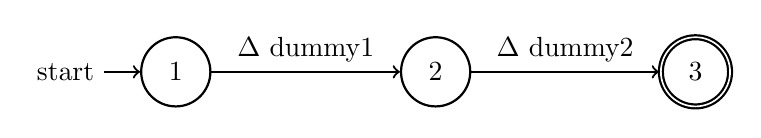
\begin{tikzpicture}[node distance={33mm}, thick, main/.style = {draw,circle}] 
          \node[initial, state] (n_1) {1};
          \node[state] (n_2) [right of=n_1] {2};
          \node[state,accepting] (n_3) [right of=n_2] {3};
          
          \draw[->] (n_1) -- node[midway, above, pos=0.5] {$\Delta$ dummy1} (n_2);
          \draw[->] (n_2) -- node[midway, above, pos=0.5] {$\Delta$ dummy2} (n_3);
        \end{tikzpicture}
    }
    \caption{Local view of the \texttt{main} actor}
    \label{local:main}
\end{figure}

\begin{figure}[!ht]
    \centering
    \resizebox{.8\textwidth}{!}{%
        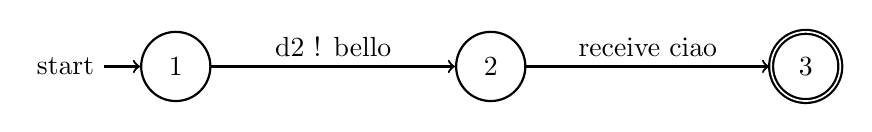
\begin{tikzpicture}[node distance={40mm}, thick, main/.style = {draw,circle}] 
          \node[initial, state] (n_1) {1};
          \node[state] (n_2) [right of=n_1] {2};
          \node[state, accepting] (n_3) [right of=n_2] {3};
          
          \draw[->] (n_1) -- node[midway, above, pos=0.5] {d2 ! bello} (n_2);
          \draw[->] (n_2) -- node[midway, above, pos=0.5] {receive ciao} (n_3);
        \end{tikzpicture}
    }
    \caption{Local view of the \texttt{dummy1} actor}
    \label{local:dummy1a}
\end{figure}

\begin{figure}[!ht]
    \centering
    \resizebox{.8\textwidth}{!}{%
        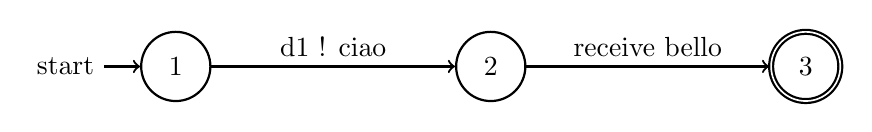
\begin{tikzpicture}[node distance={40mm}, thick, main/.style = {draw,circle}] 
          \node[initial, state] (n_1) {1};
          \node[state] (n_2) [right of=n_1] {2};
          \node[state, accepting] (n_3) [right of=n_2] {3};
          
          \draw[->] (n_1) -- node[midway, above, pos=0.5] {d1 ! ciao} (n_2);
          \draw[->] (n_2) -- node[midway, above, pos=0.5] {receive bello} (n_3);
        \end{tikzpicture}
    }
    \caption{Local view of the \texttt{dummy2} actor}
    \label{local:dummy2a}
\end{figure}

After associating the local views with the actors, the algorithm generates 
the global view shown in Figure \ref{global:async}. 
The automaton expresses two possible global 
executions of the program: from State 1 to State 3, the actors \texttt{dummy1} 
and \texttt{dummy2} are spawned. Then, since the \textit{send} operation is 
non-blocking, either \texttt{dummy1} sends \texttt{ciao} first (leading to 
State 6) or \texttt{dummy2} sends \texttt{bello} first (leading to State 4). 
Consequently, the final state is reached through two possible paths, 
depending on the order in which messages are received.

\begin{figure}[!ht]
    \centering
    \resizebox{\textwidth}{!}{%
        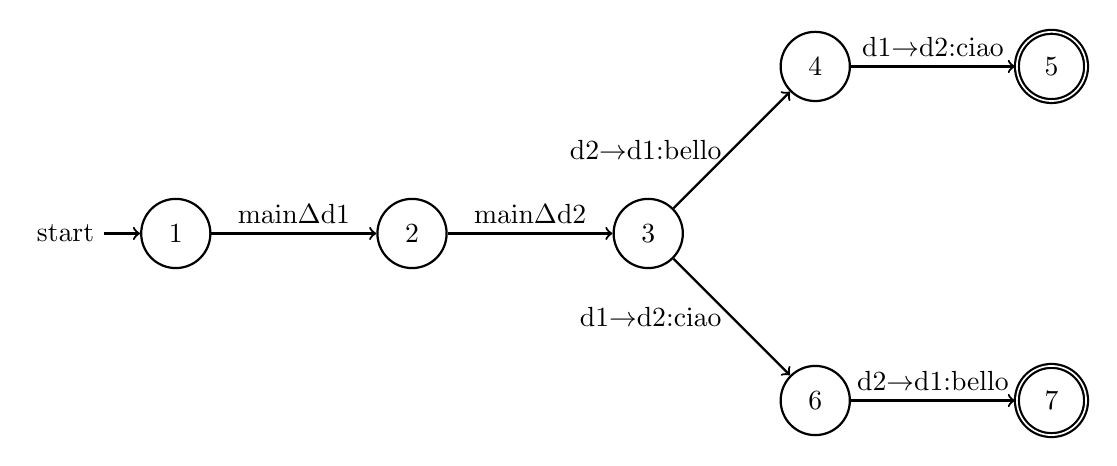
\begin{tikzpicture}[node distance={30mm},thick,main/.style={draw,circle}] 
          \node[initial, state] (n_1) {1};
          \node[state] (n_2) [right of=n_1] {2};
          \node[state] (n_3) [right of=n_2] {3};
          \node[state] (n_4) [above right of=n_3] {4};
          \node[state,accepting] (n_5) [right of=n_4] {5};
          \node[state] (n_6) [below right of=n_3] {6};
          \node[state,accepting] (n_7) [right of=n_6] {7};
          
          \draw[->] (n_1) -- node[midway, above, pos=0.5] {main$\Delta$d1} (n_2);
          \draw[->] (n_2) -- node[midway, above, pos=0.5] {main$\Delta$d2} (n_3);
          \draw[->] (n_3) -- node[midway, left, pos=0.5] {d2$\to$d1:bello} (n_4);
          \draw[->] (n_4) -- node[midway, above, pos=0.5] {d1$\to$d2:ciao} (n_5);
          \draw[->] (n_3) -- node[midway, left, pos=0.5] {d1$\to$d2:ciao} (n_6);
          \draw[->] (n_6) -- node[midway, above, pos=0.5] {d2$\to$d1:bello} (n_7);
        \end{tikzpicture}
    }
    \caption{Global view of Listing \ref{code:async}}
    \label{global:async}
\end{figure}
\end{exmp}


% inserire in appendice le definizioni, la grammatica, algoritmi
% riassumere le cose già esistenti nella parte old
% link all'appendice per le versioni formali

% riassumi molto description of tool perché lavoro precedente
% mettere insieme feature and bugs in improvments ed estendere feature
% esempi che fanno vedere le differenze tra il prima e il dopo

\subsection{Description of the tool}
\paragraph{How to use the tool}
The easiest way to use the tool is from the command line interface (CLI)
using the help of \texttt{rebar3}, a standard build tool that provides various features
such as package management for community-created libraries, compilation, and
automated project testing. By cloning the project from the public GitHub
repository and running the \texttt{rebar3 escriptize} command in the main
directory, \texttt{rebar3} will, in this order, check for and download
dependencies if needed, compile the project. After
that, an executable can be used in \texttt{./\_build/default/bin/chorer}.

\begin{lstlisting}[caption=Usage message]
Usage:
  chorer <input> <entrypoint> <output> <ming> <gstate> <minl>

Extract a choreography automata of an Erlang program.

Arguments:
  input      Erlang source file (string)
  entrypoint Entrypoint of the program (atom)
  output     Output directory for the generated dot files (string), default: ./
  ming       Minimize the globalviews , default: false
  gstate     Global state are formed with previous messages , default: true
  minl       Minimize the localviews , default: true
\end{lstlisting}

\noindent The mandatory arguments are:
\begin{itemize}
    \item \textbf{Input}: The relative path string of the input Erlang program,
    from which the tool will generate local and global views.
    \item \textbf{Entrypoint}: The atom representing the function where the
    execution of the input program begins. This parameter is essential because
    Erlang does not have a conventional entry point function (i.e. the main in C,
    but in Erlang can be every exported function). It will be passed to the
    function that creates the global view to start the simulation.
\end{itemize}

\noindent The optional arguments are:
\begin{itemize}
    \item \textbf{Output}: The relative path string of the output folder where
    the local and global view files will be saved. Local views will be named
    \texttt{[function name with arity]\_local\_view.dot}, while the global view
    file will be named \texttt{[Entrypoint]\_global\_view.dot}.
    \item \textbf{Options}: other arguments are specific operation to perform
    on the local view or the global view, i.e. produce in as output the
    minimized version of a graph.
\end{itemize}

\subsubsection{From Erlang to Choreographies}
\label{sec:corrisp}

\paragraph{Localview}

The code of a \texttt{receive} operation corresponds to the Figure \ref{grafo:receive}:
each branch will be evaluated recursively, continuing the construction from the 
branches. Finally, all branches will merge into a common node with $\epsilon$ 
transitions, from which the evaluation of the local view will resume.  
The send operation (\texttt{Pid ! message}) operation corresponds to Figure \ref{grafo:send}.  
The \texttt{spawn} function call corresponds to Figure \ref{grafo:spawn}.  

\begin{figure}[!ht]
    \centering
    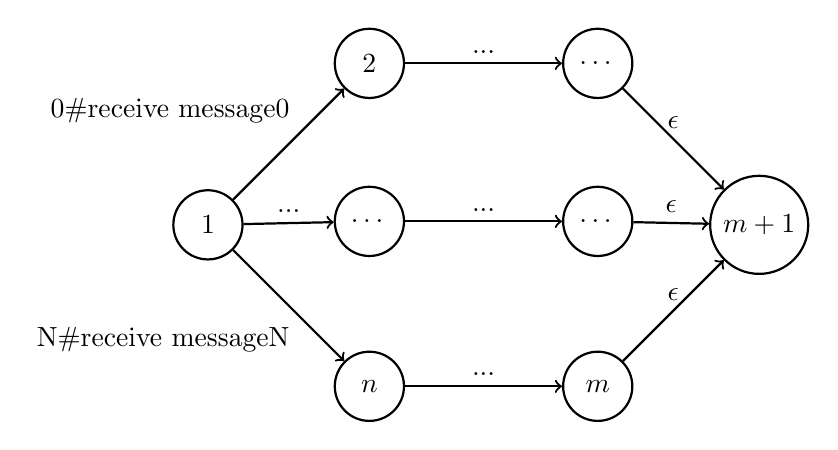
\begin{tikzpicture}[node distance={29mm}, thick, main/.style = {draw, circle}] 
      \node[state] (n_1) {1};
      \node[state] (n_2) [above right of=n_1] {2};
      \node[state] (n_4) [below right of=n_1] {$n$};
      \node[state] (n_3) [below=1.1\distance cm of n_2] {\ldots};
      \node[state] (n_5) [right of=n_2] {\ldots};
      \node[state] (n_6) [right of=n_3] {\ldots};
      \node[state] (n_7) [right of=n_4] {$m$};
      \node[state] (n_8) [below right of=n_5] {$m+1$};
      
      \draw[->] (n_1) -- node[midway, above left, pos=0.6] {0\#receive message0} (n_2);
      \draw[->] (n_1) -- node[midway, above, pos=0.5] {...} (n_3);
      \draw[->] (n_1) -- node[midway, below left, pos=0.6] {N\#receive messageN} (n_4);
      \draw[->] (n_2) -- node[midway, above, pos=0.5] {...} (n_5);
      \draw[->] (n_3) -- node[midway, above, pos=0.5] {...} (n_6);
      \draw[->] (n_4) -- node[midway, above, pos=0.5] {...} (n_7);
      \draw[->] (n_5) -- node[midway, above, pos=0.5] {$\epsilon$} (n_8);
      \draw[->] (n_6) -- node[midway, above, pos=0.5] {$\epsilon$} (n_8);
      \draw[->] (n_7) -- node[midway, above, pos=0.5] {$\epsilon$} (n_8);
    \end{tikzpicture}
    \caption{Localview graph for the \texttt{receive} keyword}
    \label{grafo:receive}
\end{figure}


\begin{figure}[!ht]
    \centering
    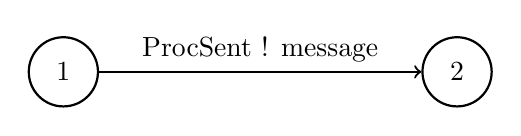
\begin{tikzpicture}[node distance={50mm}, thick, main/.style = {draw, circle}] 
      \node[state] (n_1) {1};
      \node[state] (n_2) [right of=n_1] {2};
      
      \draw[->] (n_1) -- node[midway, above, pos=0.5] {ProcSent ! message} (n_2);
    \end{tikzpicture}
    \caption{Localview graph for \texttt{!} keyword}
    \label{grafo:send}
\end{figure}

\begin{figure}[!ht]
    \centering
    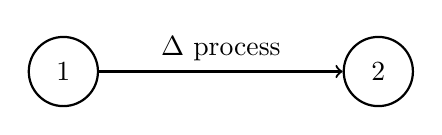
\begin{tikzpicture}[node distance={40mm}, thick, main/.style = {draw, circle}] 
      \node[state] (n_1) {1};
      \node[state] (n_2) [right of=n_1] {2};
      
      \draw[->] (n_1) -- node[midway, above, pos=0.5] {$\Delta$ process} (n_2);
    \end{tikzpicture}
    \caption{Localview graph for the \texttt{spawn} function}
    \label{grafo:spawn}
\end{figure}

\paragraph{Recursive calls}
In the case of \textit{recursive} calls, a transition $\epsilon$ is created from the last  
node generated to the first node, as shown in Figure \ref{grafo:ricors}.
For now, further evaluation of the function is blocked.

\begin{figure}[!ht]
    \centering
    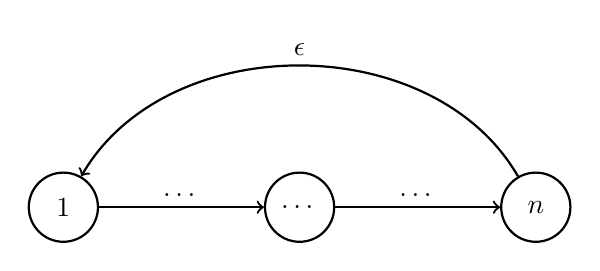
\begin{tikzpicture}[node distance={3cm}, thick, main/.style = {draw, circle}] 
      \node[state] (n_1) {1};
      \node[state] (n_2) [right of=n_1] {\ldots};
      \node[state] (n_3) [right of=n_2] {$n$};
      
      \draw[->] (n_1) -- node[midway, above, pos=0.5] {\ldots} (n_2);
      \draw[->] (n_2) -- node[midway, above, pos=0.5] {\ldots} (n_3);
      \draw[->] (n_3) to [out=120,in=60] node[midway, above, pos=0.5] {$\epsilon$} (n_1);
    \end{tikzpicture}
    \caption{Localview graph for a recursive call}
    \label{grafo:ricors}
\end{figure}

\paragraph{Function call}
When a call to an unknown function is encountered, the algorithm will create the local  
view of the called function and "connect" the beginning of the graph of the called  
function with the last state created in the local view of the calling function, linking  
them with an $\epsilon$ transition. The local view will continue from the last vertex of  
the call graph.

\begin{figure}[!ht]
    \centering
    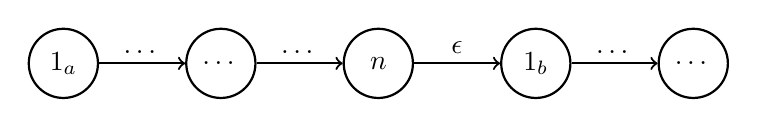
\begin{tikzpicture}[node distance={2cm}, thick, main/.style = {draw, circle}] 
      \node[state] (n_1) {$1_a$};
      \node[state] (n_2) [right of=n_1] {\ldots};
      \node[state] (n_3) [right of=n_2] {$n$};
      \node[state] (n_4) [right of=n_3] {$1_b$};
      \node[state] (n_5) [right of=n_4] {\ldots};
      
      \draw[->] (n_1) -- node[midway, above, pos=0.5] {\ldots} (n_2);
      \draw[->] (n_2) -- node[midway, above, pos=0.5] {\ldots} (n_3);
      \draw[->] (n_3) -- node[midway, above, pos=0.5] {$\epsilon$} (n_4);
      \draw[->] (n_4) -- node[midway, above, pos=0.5] {\ldots} (n_5);
    \end{tikzpicture}
    \caption{Localview graph of a function call}
    \label{grafo:funcall}
\end{figure}

In graph \ref{grafo:funcall}, state $1_a$ is the initial state of the calling function,  
and state $1_b$ represents the first state of the local view of the called function.

\paragraph{Global view}
For global views, in \texttt{spawn}, the actor performing the operation is specified to  
the left of the symbol, as shown in Figure \ref{grafo:globspawn}. A spawn will be  
directly inserted into the graph. Each process will also be numbered in case multiple  
actors are created for the same function.

\begin{figure}[!ht]
    \centering
    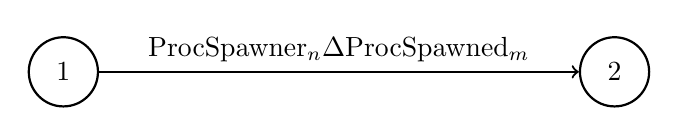
\begin{tikzpicture}[node distance={7cm}, thick, main/.style = {draw, circle}] 
      \node[state] (n_1) {1};
      \node[state] (n_2) [right of=n_1] {2};
      
      \draw[->] (n_1) -- node[midway, above, pos=0.5] {ProcSpawner$_n\Delta$ProcSpawned$_m$} (n_2);
    \end{tikzpicture}
    \caption{Global view graph for the \texttt{spawn} function}
    \label{grafo:globspawn}
\end{figure}

For message sending and receiving, during the simulation of actors, if two actors are  
found executing a compatible \textit{send} and \textit{receive}, a state will be added  
to the global view as shown in Figure \ref{grafo:sendrecv}. To be compatible, the  
receiving process must match the data recipient, and the pattern matching of the  
\textit{receive} must correspond to the sent data. Transitions for \textit{send} and  
\textit{receive} that are ``empty" (i.e., messages that are sent but not processed by a  
\textit{receive} in any process) will not be shown in the global automaton.

\begin{figure}[!ht]
    \centering
    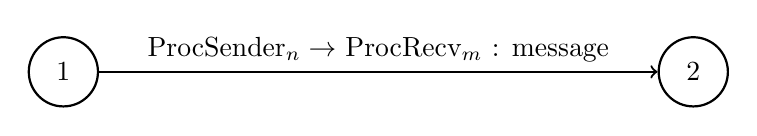
\begin{tikzpicture}[node distance={8cm}, thick, main/.style = {draw, circle}] 
      \node[state] (n_1) {1};
      \node[state] (n_2) [right of=n_1] {2};
      
      \draw[->] (n_1) -- node[midway, above, pos=0.5] {ProcSender$_n\to$ ProcRecv$_m$ : message} (n_2);
    \end{tikzpicture}
    \caption{Global view graph for \texttt{receive} and \texttt{!} keywords}
    \label{grafo:sendrecv}
\end{figure}


\subsubsection{Main algorithms}
\noindent The execution is divided into four main phases:
\begin{enumerate}
\item Initialization of the \texttt{db\_manager}, data structures, and
extraction of preliminary information (handled by the
\texttt{md.erl} module). Possible actors are extracted from
the \texttt{export} attribute, the number of \texttt{spawn}
executions is counted, and the ASTs of all functions are saved in
the \texttt{db\_manager}. Meanwhile, an initial evaluation of the
program flow is performed by initializing the names of actors and
saving the argument passing to the \texttt{spawn} functions.

\item Creation of local views for all possible actors, i.e., all functions
that appear in the \texttt{export} at the beginning of a program
(obtained from the first phase). This phase essentially acts as a compiler, 
translating Erlang programs into local choreographies.

\item Creation of the global view starting from the program's starting
point and combining the local views created in phase two.

\item Post-processing of the local and global view, inferring information on the
graph and extracting data useful for the benchmarks
\end{enumerate}

While creating a local view follows the function code line by line, the global  
view must compose local views while considering the created actors. An  
approximate execution is simulated from the startup function using the actor  
philosophy. Each actor has a manager process that tracks available transitions  
and the process state (i.e., local variables). This function provides the main  
process of the global view with actor-related information. Messages may travel  
within the same virtual machine or across a network, making message exchange  
asynchronous. If two sends, $A$ and $B$, target the same process, their order  
is unpredictable, altering the program flow.  

The global view creation algorithm follows an overapproximation approach,  
combining local views while dynamically creating communicating actors and  
exchanging messages. It explores all possible executions by handling forks in  
local views and evaluating message reception. A branch duplicates and takes  
another path in three cases: encountering a fork in a local view, multiple  
processes ready to receive, and evaluating message reception within a process.  
This ensures a thorough exploration of execution paths.  

The strategy for composing local views is to have all actors continue until  
any \textit{receive} is encountered. While searching for the first \textit{receive},  
\textit{spawn} and \textit{send} operations are also checked. If a \textit{spawn}  
occurs, the node is added to the graph, and the actor is created. If a  
\textit{send} occurs, the message is enqueued in the target process' message  
queue. After blocking on a \textit{receive}, possible messages are processed,  
creating a new execution path for each, adding new states to the global graph.  

The algorithm runs recursively until a relevant state change occurs. When an  
iteration fails to modify any actor's state, execution stops. The final graph  
represents asynchronous communication among actors for messages exchanged.  


\section{Contributions}
While the previous section discussed the basics of the tool, most of its  
content was already available at the beginning of this project. In contrast,  
this section focuses on the new contributions made to enhance the  
tool. We detail the improvements, additional features, and  
optimizations introduced, highlighting their impact on usability,  
performance, and functionality.
\subsection{Attributed grammar}
At the beginning of this period, it was challenging to clearly define the role
of the parser. There was no formal specification outlining how the tool should
process a program during its initial analysis. This lack of clarity led to
difficulties in understanding the expected behavior and designing a structured
approach for parsing.
To address this, we first examined the tool's existing implementation and
identified key areas requiring specification. Establishing a well-defined set
of rules became essential for ensuring consistent behavior and improving the
accuracy of the parsing process. Through iterative refinement, we aimed to
create a structured framework that guides the tool in extracting meaningful
information from the program.
Therefore, to better
understand how the parsing of a file and the creation of a localview 
should work, we created an attributed grammar for a subset of the Erlang 
language. An attributed grammar extends a context-free grammar by associating 
attributes with its symbols and defining semantic rules. Attributes can be 
\textit{synthesized} (computed from child nodes) or \textit{inherited}
(passed from parent nodes). 

The attribute part can be seen as a set of operations that the compiler  
performs during its analysis. This serves two key purposes: it provides  
a clear understanding of what the tool can parse from the programming  
language, and it defines how information propagates through the parse  
tree. This propagation helps identify the core data structures that  
underpin the tool’s functionality.  

The following attributed grammar will be presented alongside comments  
to provide insights into the tool’s behavior. First, we introduce the  
grammar fragment, followed by the corresponding operations applied  
to the local view data structure. These operations illustrate how the  
tool processes and interprets parsed elements, highlighting its  
internal mechanisms. 

The \texttt{link} function is used to establish a logical connection  
between two nodes. Its third argument defines the label of the transition.  
If this argument is not provided, the transition is considered an  
$\epsilon$-transition, representing an unlabeled connection. 

\paragraph{Program} For simplicity, we consider an Erlang program as a set 
of one or more functions, that can be called by the user. All the needed 
function are within the program.

\bigskip

\noindent $prog \to (function)^+$

\bigskip

A complete program does not have a local view, so there is no need  
to define attributes.  

\paragraph{Function}  
A function can have its own local view representation.  
In Erlang, pattern matching allows multiple definitions,  
so we must distinguish between the base case and the  
pattern matching case. The base case is straightforward,  
so we only present the pattern matching case.  

\bigskip

\noindent Base case: $function \to fun.$

\noindent With multiple definitions: $function \to fun_1;...;fun_N.$

\begin{verbatim}
function.nodes = new U fun1.nodes U ... U funN.nodes
function.edges = link(new,fun1.first) U ... U 
                 link(new,funN.first) U 
                 fun1.edges U ... U funN.edges
function.first = new
\end{verbatim}

Each definition has its own local view representation, so we must link  
each one to a new state. This state serves as the starting point of  
the entire local view. The nodes consist of all other nodes, and  
the same applies to the edges.  

\paragraph{Function body}  
The body of a function consists of a name (which is an atom),  
a set of arguments (which may be empty), and a list of expressions.  

\bigskip

\noindent $fun \to Atom(X_1,...,X_n) \to Exprs$

\begin{verbatim}
fun.nodes = Exprs.nodes
fun.edges = Exprs.edges
fun.first = Exprs.first
fun.last = Exprs.last
fun.context = [ X1 -> Param[1], ..., Xn -> Param[n] ]
fun.ret_var = Exprs.ret_var
\end{verbatim}

When encountering a function, we simply add its arguments to the context.  
The \texttt{Param} is taken as input, with a default value of \texttt{ANYDATA}.  
Additionally, we can perform semantic checks to verify the function’s  
existence.  

\paragraph{Expressions}  
A list of expressions can have one or more elements. The single-expression  
case is straightforward, so its attributes are omitted.  

\bigskip

\noindent Base case: $Exprs \to expr$

\noindent With multiple expression: $Exprs \to expr,Exprs'$

\begin{verbatim}
Exprs.nodes = expr.nodes U Exprs'.nodes
Exprs.edges = expr.edges 
              U Exprs'.edges 
              U link(expr.last, Exprs'.first)
Exprs.first = expr.first
Exprs.last = Exprs'.last
Exprs.context = expr.context U Exprs'.context
Exprs.ret_var = Exprs'.ret_var
\end{verbatim}

Expressions represent the lines of code in an Erlang program.  
We cover only the essential ones (e.g., assignments, function calls)  
and those related to communication.  

\paragraph{Send}   
As mentioned earlier, a send should add a transition to the local graph.  

\bigskip

\noindent $expr \to expr'\ \ !\ \ expr''$

\begin{verbatim}
expr.nodes = expr'.nodes U expr''.nodes U new1 U new2
expr.edges = expr'.edges U expr''.edges
             U link(expr'.last, expr''.first)
             U link(expr''.last, new1)
             U link(new1, new2, expr'.ret_var 
                  + " ! " 
                  + expr''.ret_var)
expr.first = expr'.first
expr.last = new2
expr.context = expr'.context U expr''.context
expr.ret_var = expr''.ret_var
\end{verbatim}

In Erlang, both the left-hand side and right-hand side of an operation  
can be expressions. First, the left-hand side expression is evaluated,  
followed by the right-hand side. Finally, a send edge is inserted with  
the corresponding variable as the label. The left-hand side must contain  
a process identifier.  

\paragraph{Receive}  
Like for a send, a receive operation should add a transition to  
the local graph for each matching pattern.  

\bigskip

\noindent $expr \to receive patter_1 \to Exprs_1; ...; pattern_n \to Exprs_n end$

\begin{verbatim}
expr.first = new1
expr.last = new2
expr.nodes = Exprs1.nodes U ... U Exprsn.nodes U new1 U new2
expr.edges = Exprs1.edges U ... U Exprsn.edges
             U link(new1, Exprs1.first) 
             U ...
             U link(new1, Exprsn.first)
             U link(Exprs1.last, new2)
             U ...
             U link(Exprsn.last, new2, espilon)
\end{verbatim}

A \texttt{receive} operation can contain an entire block of code 
that must be evaluated.  
Its return data cannot be determined statically, as it varies depending  
on the matching pattern during the global view phase. Additionally,  
since the context is modified during global view simulation,  
we leave these two attributes unchanged.  

\paragraph{Spawn call}  
The same reasoning used before applies to the \texttt{spawn} function.  

\bigskip

\noindent $expr \to spawn(Atom, Params)$

\begin{verbatim}
expr.nodes = new1 U new2
expr.edges = link(new1, new2, "spawn Atom")
expr.first = new1
expr.last = new2
expr.ret_var = newVar(type: pid, value: random) 
\end{verbatim}

The \texttt{spawn} function returns a new variable as output.  
Its type should be \texttt{pid}, with no assigned name.  
An additional logical identifier is included to differentiate  
it during global view construction. The context is left untouched
as it's not modified.

\paragraph{Recursive call}  
Recursive calls must be considered, as they are fundamental  
in functional languages like Erlang.  

\bigskip

\noindent $expr \to FunName(Params)$

\begin{verbatim}
expr.edges = expr.edges U link(FunName.first, expr.last)
expr.ret_var = null
\end{verbatim}

For recursive calls, the last added node must be linked to the first  
node of the local view being created. Using the function name,  
we can retrieve its previously created first node.  
Since a single analysis cannot determine the function's return type,  
we set the return variable to \texttt{null}. After evaluating the  
recursive call, the analysis stops, allowing only tail-recursive  
functions.  

\paragraph{Generic function call}  
To complete the previous analysis, we define attributes for  
standard function calls.  

\bigskip

\noindent $expr \to Atom(Params)$

\begin{verbatim}
G = get_localview(Atom, Param)
expr.nodes = G.nodes
expr.edges = G.edges
expr.first = G.first
expr.last = G.last
expr.ret_var = G.ret_var 
\end{verbatim}

With \texttt{get\_localview}, we retrieve the necessary information  
to complete the local view for a generic function call.  

\paragraph{Assignment}  
Finally, assignments must be handled to support basic programs  
with variables. Assignments in Erlang are peculiar as it has
immutable variables: they behave  
as pattern matching when a variable is already defined.
Thus, semantic checks can be performed.  

\bigskip

\noindent $expr \to pattern = expr'$

\begin{verbatim}
expr.nodes = expr'.nodes
expr.edges = expr'.edges
expr.first = expr'.first
expr.last = expr'.last
expr.context = [pattern -> expr'.ret_var]
\end{verbatim}

The pattern should add the new variable to the context  
with its assigned name.  

\paragraph{Conclusion}
We defined the attributed grammar for the \texttt{localview} module of our tool.  
This process highlighted the need for a \texttt{localview} with the following  
attributes: \texttt{nodes} and \texttt{edges}, with labels to represent the  
automaton; a \texttt{first} and \texttt{last} node to track entry and exit  
points; and a \texttt{context} along with \texttt{ret\_var} for basic  
variable management.
Some of these attributes are already present in the current codebase,  
but their handling differs, and additional arguments must be incorporated.  
Thus, a refactoring process is required to align the implementation with  
this attributed grammar.

This technique is particularly powerful in our case. 
For instance, a known issue with  
mutual recursive functions can be effectively addressed by improving  
context management inspired by the attributed grammar.
Using this method extensively could be key to  
efficiently representing \texttt{localviews}. 
However, the refactoring process is extensive and time-consuming.  
Therefore, it has been identified as a high-priority task for future work.  



\subsection{Improvements on the tool}
One key goal of the tool is to generate correct graph outputs, ensuring an  
accurate representation of program behavior. While refining abstract aspects  
of the project, several features, improvements, and bug fixes have been added  
to enhance the precision and consistency of the global view specification. The  
iterative process of refining the tool aims to minimize errors, and provide a
more reliable emulation of  actor-based execution. Future work will continue to
focus on refining these aspects to offer greater 
flexibility while maintaining correctness of the analyzed program.

\paragraph{Features}
Two key features have been added to the tool. The first one improves the local  
view module. The tool can now correctly parse programs where values are passed   
as arguments to functions, allowing for a more precise representation of  
data flow between processes. 
Previously, only functions without value passing were supported. This was a
significant limitation and, in fact, one of the highest-priority features.
It was the final major feature of a programming language to be added, and it is 
now included in the parsing module, enabling a broader range of program inputs.

The second feature added to the tool enhances over-approximation
in the global view module. During computation, the value of 
some data can become everything because we cannot know the outcome of an 
operation performed on the data (i.e. we don't support mathematical operation). 
The tool now substitutes this unknown value with the \texttt{ANY} keyword to 
indicate that it can represent any kind of data. If a message is exchanged with 
\texttt{ANY} as its content, it will match every possible receive branch,
ensuring a more over-approximated analysis of the program.

\paragraph{General improvements}
Some general improvements have been made on the tool. 
The tool is now more resilient to unexpected errors, reducing the  
likelihood of crashes and ensuring that it provides meaningful output in  
most cases, even when encountering invalid input. This was achieved through the
implementation of more error checks and recovery patterns within the codebase, 
where there were none before.

Also, a new library has been integrated for command-line argument management,  
making the CLI more robust and user-friendly, with better parsing of  
parameters and improved error messages.

Some effort has been put to improve the testing environment and benchmark 
generation. The tool now produces useful benchmarking information, which is 
processed by a dedicated Python script. This script collects and analyzes the 
data to generate meaningful performance benchmarks. Additionally, if the  
\texttt{correct\_gv.dot} file is present (that is a dot file containing 
the expected global view) the script performs an automatic correctness check. 
This feature lays the groundwork for more expressive and rigorous testing in 
the future, enabling better validation of the tool's accuracy and performance
across different scenarios and use cases.

\paragraph{Bug fixes}
Some notable bug fix improvements were made within the global view module that 
are needed to be mentioned. It has been resolved an issue where the tool
incorrectly printed warnings about failing to find the correct process during
the sending of a message. This bug caused the useless show of some false 
positive warnings. 

It also has been addressed a problem that prevented the exploration of certain
branches during the global view emulation, ensuring a more comprehensive
traversal of all possible execution paths. This bug prevented a full branch
exploration in certain programs. 

It has been fixed a bug that was causing the creation of excessive duplicated
branches. This patch corrected an issue where unnecessary duplicated branches 
were created after receiving a message and defining a new variable. This fix
improves the accuracy of the global view by reducing redundant computations.  


\subsection{Benchmarks}
\begin{table}[!ht]
\centering
\begin{tabular}{|c|c|c|c|c|c|c|}
\hline
Example & Lines & GV Nodes & GV Edges & Warnings & Errors & Runtime \\ 
\hline
account & 23 & 19 & 27 & 0 & 2 & 0.261s \\ 
dining & 31 & 29 & 44 & 0 & 2 & 0.250s \\ 
hello & 24 & 3 & 3 & 2 & 0 & 0.189s \\ 
async & 20 & 6 & 6 & 0 & 0 & 0.188s \\ 
ticktackstop & 46 & 12 & 19 & 7 & 0 & 0.210s \\ 
ticktackloop & 32 & 5 & 5 & 2 & 0 & 0.184s \\ 
customer & 54 & 12 & 16 & 1 & 0 & 0.209s \\ 
serverclient & 41 & 7 & 8 & 8 & 3 & 0.193s \\ 
trick & 24 & 8 & 8 & 0 & 0 & 0.185s \\ 
airline & 23 & 12 & 20 & 1 & 0 & 0.225s \\ 
conditional-case & 26 & 10 & 15 & 1 & 16 & 0.198s \\ 
for-loop-recursion & 18 & 8 & 9 & 0 & 0 & 0.186s \\ 
function-call & 17 & 3 & 3 & 1 & 2 & 0.184s \\ 
high-order-fun & 21 & 10 & 14 & 0 & 3 & 0.193s \\ 
if-cases & 57 & 86 & 134 & 185 & 30 & 0.543s \\ 
pass & 16 & 3 & 2 & 0 & 0 & 0.196s \\ 
producer & 30 & 8 & 7 & 0 & 1 & 0.198s \\ 
spawn & 22 & 9 & 8 & 0 & 0 & 0.182s \\ 
unknown & 13 & 1 & 1 & 0 & 0 & 0.187s \\ 
foo1 & 18 & 6 & 7 & 0 & 0 & 0.215s \\ 
foo2 & 23 & 4 & 3 & 1 & 1 & 0.190s \\ 
foo3 & 22 & 10 & 14 & 0 & 0 & 0.195s \\ 
foo4 & 20 & 12 & 15 & 0 & 2 & 0.194s \\ 
foo5 & 18 & 39 & 87 & 1 & 0 & 0.317s \\ 
foo6 & 24 & 6 & 7 & 15 & 2 & 0.200s \\ 
foo7 & 41 & 43 & 121 & 0 & 6 & 0.520s \\ 
foo8 & 29 & 27 & 95 & 0 & 171 & 2.893s \\ 
foo9 & 14 & 2 & 3 & 1 & 3 & 0.191s \\ 
foo9b & 21 & 4 & 4 & 14 & 1 & 0.188s \\ 
foo9c & 15 & 6 & 11 & 0 & 0 & 0.198s \\ 
foo9d & 16 & 3 & 2 & 0 & 0 & 0.186s \\ 
foo9e & 24 & 9 & 13 & 0 & 5 & 0.193s \\ 
foo9f & 25 & 4 & 6 & 0 & 4 & 0.193s \\ 
foo9g & 25 & 21 & 49 & 0 & 7 & 0.231s \\ 
foo9h & 23 & 12 & 26 & 0 & 5 & 0.196s \\ 
ping & 36 & 6 & 5 & 1 & 0 & 0.183s \\ 
airline & 33 & 18 & 34 & 1 & 0 & 0.225s \\ 
meViolation & 40 & 38 & 54 & 2 & 4 & 0.255s \\ 
purchase & 47 & 25 & 44 & 6 & 0 & 0.254s \\ 
\hline
\end{tabular}
\caption{Global view data}
\label{tab:gvbench}
\end{table}



\section{Case studies}
In order to better illustrate our point, we present in this section two examples (using Erlang-like, actor-based pseudocode), each one
composed by a pseudocode and the corresponding Choreography
Automaton~\cite{coordination2020-chorAuto} (a graphical way of
representing a finite-state machine) of the global view of the
communicating system. Here, a \emph{global view} is an abstract description of
all the possible behaviors of the full system. We consider a language
where receive statements are blocking operations. A state where each
participant has completed its task and terminated is called \emph{final}. As such, a
state that is not final and has no outgoing transitions is a \emph{deadlock}.

The first example is a concise reproduction of the dining philosophers
problem, which highlights a possible deadlock. The second example
shows a possible mutual exclusion error 
when operating a simple bank account.
%in a database.
%
Both examples are available online~\cite{chorer_examples}; the
corresponding automata have been obtained with the help of our prototype tool
Chorer~\cite{chorer}.

\lstset{language=erlang, basicstyle=\sffamily\footnotesize,
  keywordstyle=\color{blue}, numberstyle=\tiny, numbers=none,
  showspaces=false, showstringspaces=false, frame=tL,
  backgroundcolor=\color{black!5}, morekeywords={send, to, from} }


In the examples, we exploit two operations for sending and receiving messages,
respectively.
%
More precisely, \lstinline[language=erlang, morekeywords={send,
  to}]{send msg to proc} sends message \lstinline{msg} to process
\lstinline{proc}, while \lstinline[morekeywords={receive,
  from}]{receive pat1 from proc1 -> e1;...;patn from procn -> en} 
  represents a branching point where the process receives 
  the first message 
  that matches a pattern $\mathsf{pati}$ and, then, 
  continues with the execution of $\mathsf{ei}$. 
  As in Erlang, 
  %we allow \lstinline[language=erlang]{receive}
%statement with multiple clauses where the 
pattern matching is tried from top to bottom.
% when there are
%multiple clauses.
When a receive has only one clause, we abbreviate it as
\lstinline[morekeywords={receive,from}]{receive pat from proc}
(and continues with the execution of the next sentence).
\subsection{Dinning philosophers}
\paragraph{Dining Philosophers Example}
This example is taken from the \texttt{dining} case study from the benchmark 
suite of the tool.
Let us consider a program with two participants playing the role of a
dining philosopher who shares two forks with the other participant.

\begin{lstlisting}
philosopher(Fork1, Fork2) ->
  send req to Fork1,
  receive ack from Fork1,
  send req to Fork2,
  receive ack from Fork2,
  eat(),
  send release to Fork1,
  send release to Fork2,
  philosopher(Fork1, Fork2).

fork() ->
  receive req from Phil,
  send ack to Phil,
  receive release from Phil,
  fork().
\end{lstlisting}
%
% Consider the following 
% %\footnote{The
% %corresponding Erlang code can be found in our
% %\href{https://github.com/gabrielegenovese/chorer/blob/example/deadlock/examples/paper_example/deadlock/deadlock.erl}{github}
% %repository.} 
% program, where each function defines the behavior of a
% participant in the communicating system, which can be instantiated
% multiple times.  The program models two dining philosophers.
%

%
The behavior of the philosophers is given by the pseudocode on the
right while pseudocode for the behavior of the forks is discussed below.
Each philosopher first acquires the forks (starting with the one on
its right, that is the one with the same index), then eats (with the
function call \lstinline{eat()} representing some terminating local
computation), and finally releases the forks before recurring.
Parameters \lstinline{Fork1} and \lstinline{Fork2} are references to
processes executing the behavior of forks described by the pseudocode on the left
that repeatedly waits for the request from process \lstinline{Phil},
\lstinline{ack}s the request, and waits for the \lstinline{release}
message from \lstinline{Phil}.


There are two possible behaviors of the system. The first (good) one where the philosophers alternate eating infinitely and a second (bad) behavior 
%three
%possible executions of the system. In the first one, the first
%philosopher takes both forks, eats, then releases them,
%allowing the second philosopher to do the same. In the second
%execution, the philosophers eat in the opposite order. Given the recursive behavior of the \texttt{philosopher} 
%function, the actors could alternate infinitely.
%In the third possible execution, 
where both philosophers
manage to take only one fork each %, but they cannot take the other, as they
%are waiting for the other philosopher to release it. This 
resulting in a deadlock. 
Figure~\ref{graph:philosophers} depicts the global Choreography Automaton
representing the program above. 
We have two recursive executions where both philosophers
eat, represented as loops, and two executions which end in the same
deadlock state.
%\footnote{The full global view,
%obtained with our prototype tool Chorer \cite{chorer}, can be seen in
%our
%\href{https://github.com/gabrielegenovese/chorer/blob/example/deadlock/examples/paper_example/deadlock/main_0_global_view.dot}
  %   {github} repository.}.
%
%In the automaton, State 1 is the entry point. From State 1, we have
%two possible transitions, to State 2 and State 3 respectively, which
%model the requests (\texttt{req}) of the philosophers to the forks
%with the corresponding index. The two transitions can occur in any
%order (indeed there are transitions to State 5 closing the commuting
%diamond).
%
%Transitioning from State 1 to State 2 means that the system first 
%performs the \texttt{req} communication for the first philosopher. 
%Transitioning from State 1 to State 3 means that it first performs 
%the \texttt{req} communication for the second philosopher.
%States 2 and 3 represent states where there is a race between the
%philosopher that already has one fork taking the other (transitions on
%the side, leading to a loop), or the other philosopher taking the
%fork, leading to the deadlock in State 5. 
The deadlock is 
visible since State 5 is not final, and it has no outgoing transitions.
%Also, the system has a race, this is visible in the choreography
%automaton since State 3 has two outgoing transitions with the same
%receiver (the same for State 2), but we want to see these transitions
%since some of them lead to the deadlock state. 
  The automaton is simplified %w.r.t.~a full model of the program, 
  as it does not display the \texttt{ack} messages, and the
  \texttt{release} messages are merged since their order is
  irrelevant. The focus here is solely on the order of the
  \texttt{req} messages. One can imagine to first extract the full
  choreography automaton, and then merge equivalent behaviors and abstract away from uninteresting transitions.
%  to focus on the ones of interest. 
%  Another possible simplification
%  would be to notice that the system is symmetric (w.r.t.~the swap of
%  the two philosophers), hence it would be enough to analyze one of
%  the two halves.



\begin{figure}[t]
  \centering
  % \includegraphics[scale=.35]{images/deadlock.png}
  % \makebox[\textwidth][c]{
  \resizebox{0.9\textwidth}{!}{%
      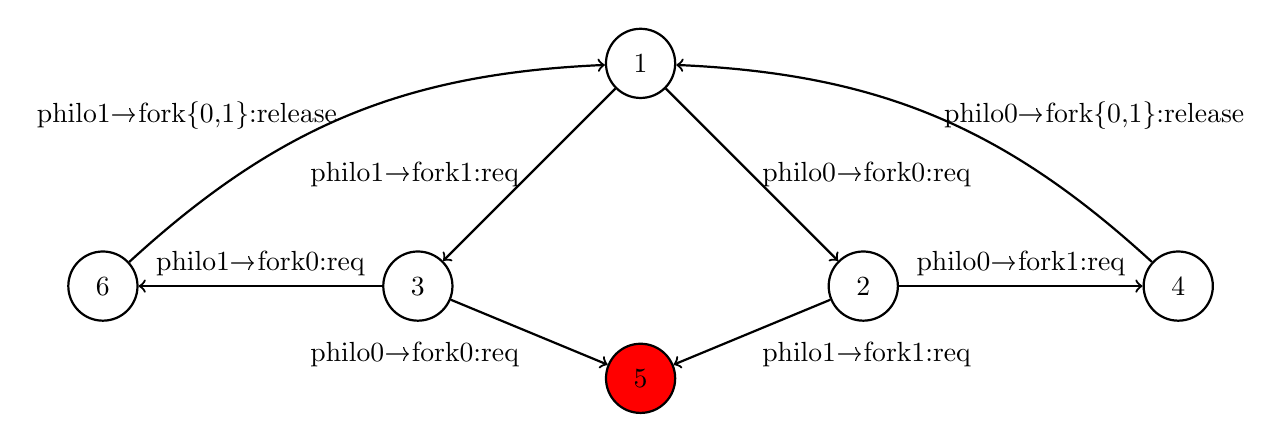
\begin{tikzpicture}[node distance={40mm}, thick, main/.style = {draw, circle}] 
        \node[state] (n_1) {1};
        \node[state] (n_2) [below right of=n_1] {2};
        \node[state] (n_3) [below left of=n_1] {3};
        \node[state] (n_4) [right of=n_2] {4};
        \node[state] (n_5) [below of=n_1, fill=red] {5};
        \node[state] (n_6) [left of=n_3] {6};
        
        \draw[->] (n_1) -- node[midway, right, pos=0.5] {philo0→fork0:req} (n_2);
        \draw[->] (n_1) -- node[midway, left, pos=0.5] {philo1→fork1:req} (n_3);
        \draw[->] (n_2) -- node[midway, below right, pos=0.5] {philo1→fork1:req} (n_5);
        \draw[->] (n_3) -- node[midway, below left, pos=0.5] {philo0→fork0:req} (n_5);
        \draw[->] (n_2) -- node[midway, above, pos=0.5] {philo0→fork1:req} (n_4);
        \draw[->] (n_4) to[bend right=20] node[midway, right, pos=0.5] {philo0→fork\{0,1\}:release} (n_1);
        \draw[->] (n_3) -- node[midway, above, pos=0.5] {philo1→fork0:req} (n_6);
        \draw[->] (n_6) to[bend left=20] node[midway, left, pos=0.5] {philo1→fork\{0,1\}:release} (n_1);
      \end{tikzpicture}
    }
  % }%
  \caption{Global view of the dining philosophers example.}
  \label{graph:philosophers}
\end{figure}
\subsection{Bank account}
This case study is taken from the \texttt{account} example from the benchmark 
suite of the tool.
We now consider a system where a bank account is accessed
by two clients, dubbed C1 and C2.
% 
\tikzset{
	hpath/.style={
			very thick,
			line cap = round,
			line join = round,
			line width=0.1cm,
			opacity=.70,
			color = teal!30
		}
}

\bigskip

\begin{lstlisting}
account(Value) ->
  receive
    read from Client ->
      send Value to Client,
      account(Value);
    NewValue from Client ->
      account(NewValue).

client() ->
  send read to Acc,
  receive Value from Acc,
  % operations on Value
  send NewValue to Acc.
\end{lstlisting}

\bigskip

The pseudocode yields the behavior of the bank account,
where $\mathsf{Value}$ represents its current balance.
This process waits for requests from a client.
A request can either be a \lstinline{read} access to know
the current balance or an update request of such value to a
\lstinline{NewValue}.

Symmetrically, client processes C1 and C2 behave according to the
pseudocode on the left: the process reads the current balance
from the account,
performs some internal operations based on such value, and
updates the balance.
%
The global view of the communicating system is depicted in
Figure~\ref{fig:account}.

\newcommand\dummy{C}
\begin{figure}[!ht]
	\centering
	\begin{tikzpicture}[node distance={27mm}, scale = .6, transform shape, thick, main/.style = {draw, circle}]
		\node (n_1) [state] {};
		\node (n_2) [state, below left of=n_1] {};
		\node (n_3) [state, below right of=n_1] {};
		\node (n_4) [state, left= 3.5cm of n_2] {4};
		\node (n_5) [state, below=3cm of n_1] {};
		\node (n_6) [state, right= 3.5cm of n_3] {6};
		\node (n_7) [state, below of=n_4] {7};
		\node (n_8) [state, below left of=n_5] {};
		\node (n_9) [state, below right of=n_5] {};
		\node (n_10) [state, below of=n_6] {10};
		\node (n_11) [state, accepting, below= of n_7] {11};
		\node (n_12) [state, accepting, below=1.5cm of n_8] {};
		\node (n_13) [state, accepting, below= 1.5cm of n_9] {};
		\node (n_14) [state, accepting, below=2.5cm of n_10] {14};

		\draw[->] (n_1) -- node[midway, above left] {acc→\dummy1:Value} (n_2);
		\draw[->] (n_2) -- node[midway, below left] {acc→\dummy2:Value} (n_5);
		\draw[->] (n_5) -- node[midway, above left=-2mm] {\dummy1→acc:NewValue} (n_8);
		\draw[->] (n_8) -- node[midway, below left] {\dummy2→acc:NewValue} (n_12);

		\draw[->] (n_1) -- node[midway, above right] {acc→\dummy2:Value} (n_3);
		\draw[->] (n_3) -- node[midway, below right] {acc→\dummy1:Value} (n_5);
		\draw[->] (n_5) -- node[midway, above right=-2mm] {\dummy2→acc:NewValue} (n_9);
		\draw[->] (n_9) -- node[midway, below right] {\dummy1→acc:NewValue} (n_13);

		\draw[hpath] ($(n_1.center) + (-5pt,-5pt)$) -- (n_2.center) -- (n_5.north west) -- ($(n_5.center)+(-5pt,0)$) -- (n_5.south west) -- (n_8.center) -- ($(n_12.center) + (0pt,5pt)$);
		\draw[hpath] ($(n_1.center) + (5pt,-5pt)$) -- (n_3.center) -- (n_5.north east)  -- ($(n_5.center)+(5pt,0)$) -- (n_5.south east)  -- (n_9.center) -- ($(n_13.center) + (0pt,5pt)$);

		\foreach \n in {1,2,3,5,8,9,12,13}{
				\node at (n_\n) {\n};
			}

		\draw[->] (n_2) -- node[midway, above=3mm] {C1→acc:NewValue} (n_4);
		\draw[->] (n_4) -- node[midway, above left] {acc→C2:Value} (n_7);
		\draw[->] (n_7) -- node[midway, above left] {C2→acc:NewValue} (n_11);

		\draw[->] (n_3) -- node[midway, above=3mm] {C2→acc:NewValue} (n_6);
		\draw[->] (n_6) -- node[midway, above right] {acc→C1:Value} (n_10);
		\draw[->] (n_10) -- node[midway, above right] {C1→acc:NewValue} (n_14);
	\end{tikzpicture}
	\caption{Global view of the bank account example}
	\label{fig:account}
\end{figure}

We can observe two correct executions where the operations are
performed in a read-update-read-update order (taking the path via
states 1-2-4-7-11 or the one via states 1-3-6-10-14).
%

However, there is also a read-read-update-update order on the
highlighted paths.
%
Although the choreography is not inherently incorrect, these
highlighted paths could represent a violation of mutual exclusion
which may be undesirable for developers in certain
contexts.
The choreography automaton in Figure~\ref{fig:account} helps in spotting
this issue.

%%% Local Variables:
%%% mode: LaTeX
%%% TeX-master: "main"
%%% End:


\section{Conclusion}
% parlare delle cose future

\subsection{Related works}
In the industrial context, Erlang's actor model has also inspired other 
programming languages or frameworks, such as Elixir \cite{website:elixir}, a 
programming language based on Erlang's virtual machine. Other programming 
languages also implement the actor model, such as Go \cite{website:golang} with 
its GoRoutines (comparable to Erlang's spawns) and channels (similar to Erlang's
send and receive).
Software industry is increasingly devoting attention to choreographic approaches
\cite{BPMN,bon18,fmmt20,DBLP:journals/software/AutiliIT15} because
they naturally support modularization and decoupling.
%
In fact, distributed components coordinate according to a global
description without the need of an explicit coordinator.
%
In the academic context, research in the field of \textit{choreography} focuses 
on two main topics: \textit{choreography specification} and 
\textit{choreographic programming}.
\begin{itemize}
    \item \textit{Choreography specifications}: this area includes formal 
    methods, such as multiparty asynchronous session types 
    \cite{honda2008multiparty}, which have been established to describe the 
    interactive structure of a fixed number of actors from a global perspective.
    These methods enable the syntactic verification of actors' correctness by 
    projecting the global specification onto individual participants. 
    Choreography specifications are also studied as contracts, which provide 
    abstract descriptions of program behavior, known as \textit{multiparty 
    contracts} \cite{zava}.
    \item \textit{Choreographic programming}: this programming paradigm has been
    explored both theoretically, as in \cite{website:wscdl}, and industrially, 
    as in \cite{website:bpmn}. Several choreographic programming languages have
    been designed and studied to support this paradigm \cite{montesi2010jolie, 
    montesi2014choreographic, giallorenzo2020object, dalla2014aiocj}.
\end{itemize}
In this context, global specifications are crucial for guaranteeing
correctness (since they are blueprints of complex distributed systems
and feature model-driven development) as well as for program
comprehension. 
Most formal works on communication protocol 
specifications emphasize the projection of a global specification onto local 
specifications. However, the process of choreography extraction remains 
challenging and has been explored in \cite{cflm17}, with a general 
framework for extracting choreographies presented in 
\cite{cruz2022implementing}.
%
To the best of our knowledge, the first attempts to extract global
specifications for message-passing systems goes back
to~\cite{myh09,lt12,lty15}.
%
These approaches aim to identify ``meaningful" global specifications
according to general properties such as deadlock-freedom or absence of
orphan messages~\cite{bz83}.
%
A limitation of these approaches is that they do not start from
components written in a full-fledged programming language.
%
Rather, distributed components are specified in~\cite{lt12,lty15} as
abstract models (respectively, $\pi$-calculus
processes~\cite{sw02,mil99,mpw92} and communicating finite-state
machines~\cite{bz83}).


%%% Local Variables:
%%% mode: LaTeX
%%% TeX-master: "main"
%%% End:


\newpage

\bibliographystyle{plain}
\bibliography{ref}

\end{document}
